\subsection{Simplified models spectra and naming conventions}
\def\chitz{\ensuremath{\widetilde{\chi}^0_2}}
\def\chiz{\ensuremath{\widetilde{\chi}^0_1}}
\def\chipm{\ensuremath{\widetilde{\chi}^\pm_1}}
\def\chimp{\ensuremath{\widetilde{\chi}^\mp_1}}
\def\gl{\tilde{g}}
\def\sTop{\ensuremath{\tilde{t}}\xspace}
\def\st{\ensuremath{\tilde{t}}\xspace}
\def\slep{\ensuremath{\tilde{l}}\xspace}
\def\snu{\ensuremath{\tilde{\nu}}\xspace}
\def\sBottom{\tilde{b}}
\def\sb{\tilde{b}}
\def\sq{\tilde{q}}
\def\sb{\tilde{b}}
\def\st{\tilde{t}}
\def\fb{\mathrm{fb}}
\def\first{1$^\mathrm{st}$}
\def\second{2$^\mathrm{nd}$\xspace}
\def\third{3$^\mathrm{rd}$\xspace}
\def\spacer{\hspace*{10mm} }
\definecolor{red}{rgb}{.6,.02,.02} 
%\newcommand\fixme[1]{{\begin{color}{red}FIXME #1\end{color}}}
\newcommand\fixme[1]{{\color{red}FIXME #1}}
\newcommand\model[1]{{\tt #1}}
\newcommand\url[1]{{\nopagebreak{\tt #1}}}
\newcommand\smallurl[1]{{\small \tt #1}}
\newcommand{\AlphaT}{\ensuremath{\alpha_{\mathrm{T}}}\xspace} 
\newcommand{\ATLLepStop}{ATL lep-$\tilde{t}$}
\newcommand{\ATLHadStop}{ATL had-$\tilde{t}$}
\newcommand{\SSnoHT}{SSnoH$_{\mathrm{T}}$}
\newcommand{\HsTjets}{\ensuremath{\not\!\!\mathrm{H}_{\mathrm{T}}}+jets\xspace}
\newcommand{\MTtwo}{\ensuremath{{M}_{\mathrm{T2}}}\xspace}  
\newcommand{\emu}{\ensuremath{e/\mu}\xspace}
\newcommand{\ETslash}{\ensuremath{\not\!\!\rm{E}_{\mathrm{T}}}\xspace} 
\newcommand{\ZMET}{Z+\ETslash}
\newcommand{\sigmaXBF}{\mbox{\ensuremath{\sigma\times\mathcal{B}}}\xspace}

\label{ssec:names}
In this document, the naming convention of Refs~\cite{SUS11016},~\cite{cms:2013wc}
will be used and extended:
All names start with a ``T'', which stands for ``topology''.  In the case of
gluino-gluino production the ``T'' is followed by an odd number,
depending on the assumption about the gluino decay. Direct decays to quarks and
the LSP are labelled ``1''; in the case of an intermediate state appearing on
one leg of the simplified model but not on the other, a ``3'' is appended,
while ``5'' denotes intermediate states on both legs. For squark-squark
production, even numbers are used: ``2'' denotes direct decay to the LSP, while
``4'' and ``6'' code for topologies with intermediate mass states on one and
two legs, respectively.  Postfixes specify details about the final states. For
example,  T1tttt represents gluino production, where both gluinos decay via
$\gl \rightarrow t t \chiz$; T2bb is sbottom-sbottom production, with sbottoms
decaying via $\sb \rightarrow b \chiz$ and TGQ codes are associated with
gluino-squark production, and TGQ* represents gluino-squark production with
intermediate mass states.  The symbol TChi denotes weakino production. The
occurence of on-shell gauge or Higgs bosons
is denoted by the ``final state''; for example,  TChiwz denotes the production
of a chargino and a heavy neutralino, where $\chipm \rightarrow W^\pm \chiz$
and $\chitz \rightarrow Z \chiz$. In the case of a three-body decay, the
weakinos are named directly: TChiC1N2 indicates the production of a chargino
(C1) and a heavy neutralino (N2).
The LSP is marked as ``N1''. See
Figs.~\ref{fig:gluinoSMSes},~\ref{fig:squarkSMSes} for examples.
\fixme{this is currently taken from the CMS-pMSSM paper.
This paragraph will need to be rewritten, once we know what SMSes we need/use.}

\subsection{Anatomy of an SMS result}
\label{ssec:smsstatistics}
As a simplified model introduces only a very limited number of new particles,
a scan in all free parameters of the simplified model can easily be performed.
The CMS and ATLAS collaborations typically use such scans to produce two types
of resulting plots: given a well-defined signal region, the collaborations
can report the analysis' acceptance times efficiency values ($A \times
\epsilon$), as a function of the mass parameters. Such a result is shown in
Fig.~\ref{fig:smsexampleeff}. 
In a second step, a 95\% confidence level upper limit (UL) on the product of
the cross section and branching fraction (\sigmaXBF) is computed, as a function
of the model's mass parameters. A typical result can be seen in
Fig.~\ref{fig:smsexampleul}: the colors show the binned values of \sigmaXBF.
In addition, the collaborations compare the values of \sigmaXBF with
theoretical ``reference'' cross sections, to draw exclusion lines, assuming a
branching ratio of $\mathcal{B}=1$. 

\begin{figure}[ht!]
\begin{center}
\begin{tabular}{lr}
\subfigure[\label{fig:smsexampleeff}efficiency plot]{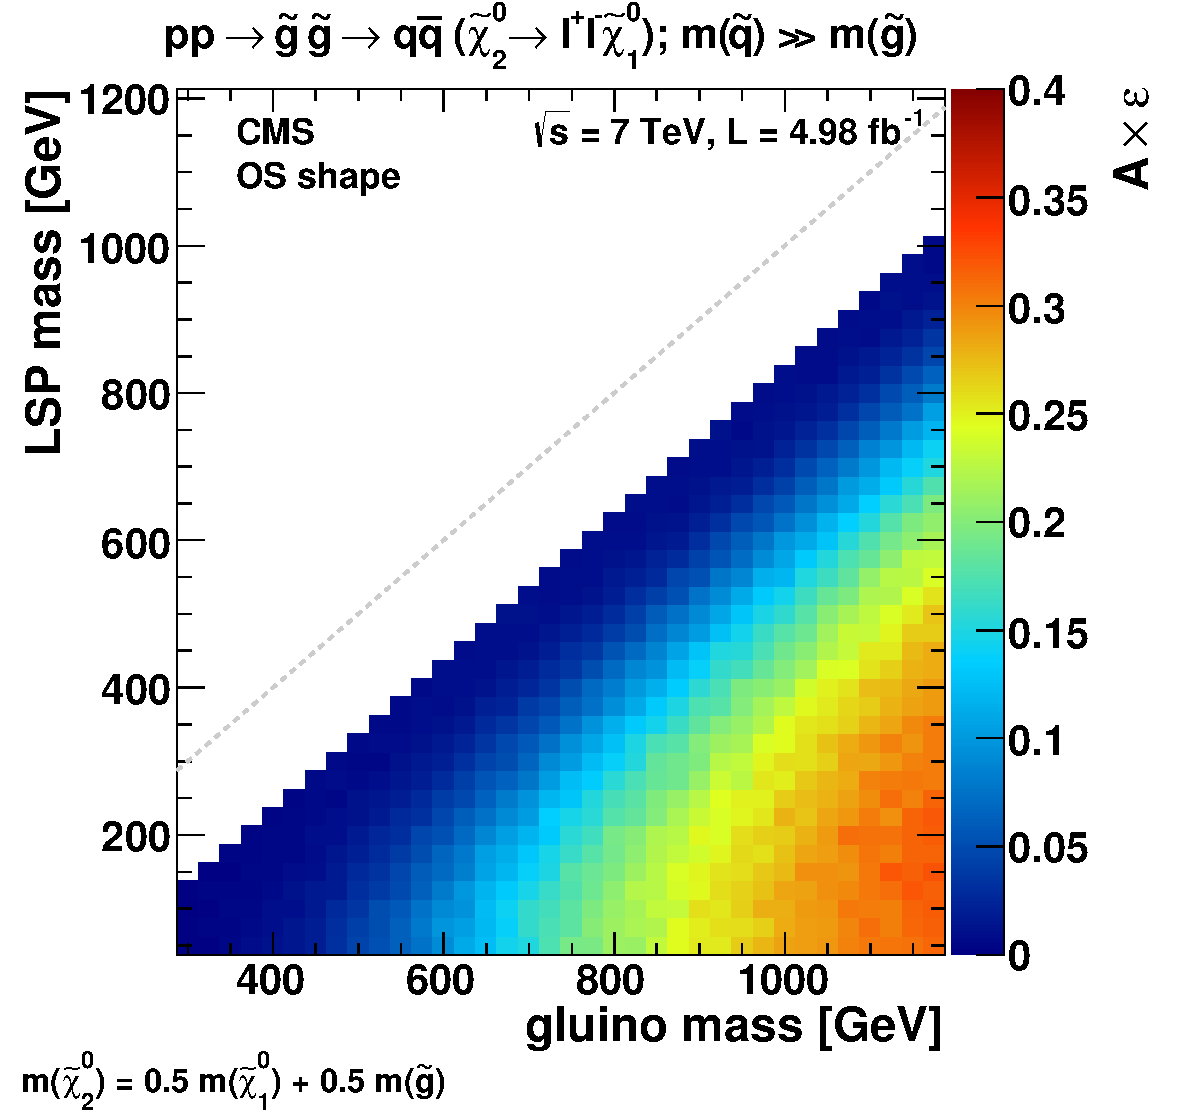
\includegraphics[width=0.5\linewidth]{figures/h_eff_T3lh_OSshape.pdf}} &
\subfigure[\label{fig:smsexampleul}upper limits on production cross
section]
{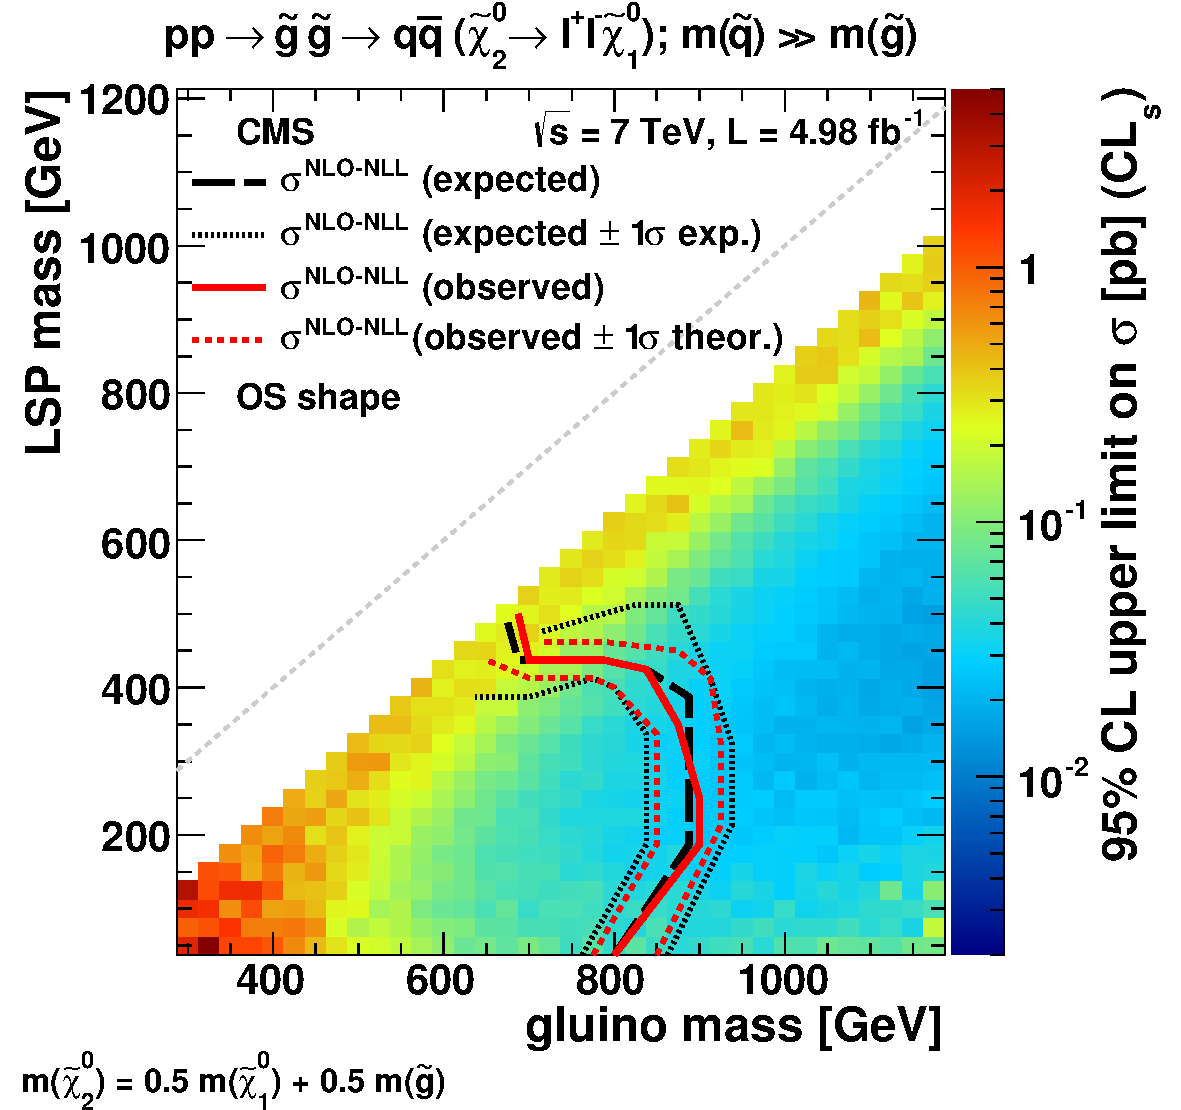
\includegraphics[width=0.5\linewidth]{figures/h_limit_T3lh_OSshape.pdf}}
\\
\end{tabular}
\caption{An example of an SMS result of the CMS collaboration, taken
from~\cite{cms:2013wc}.}
\label{fig:smsexample}
\end{center}
\end{figure}

This document builds upon the 95\% upper limits on \sigmaXBF -- neither the
efficiency plots nor the exclusion lines are of any relevance for this work.
It is however a long-standing wish of the authors to the experimental
collaborations to publish not only the 95\% upper limits, but rather the entire
likelihoods.  This would e.g. allow combinations of LHC results with
uncorrelated non-LHC measurements.  
A combination of several LHC results would still not be feasible because 
the correlations between the SMS results are unknown.
It is an even longer term vision that all ingredients that enter
into the statistical procedure are published also;
in an ideal world a user of the LHC results would be able to produce 
a likelihood for any combination of SMS results published, be they from CMS or
ATLAS.

\subsection{LHC results used}
\label{ssec:lhc}
The SMS results that are currently included in the database are:
\fixme{In the end we will need a clean up and discuss only those results that
we actually used.}
A description of many CMS results used in this document is given in
Ref.~\cite{cms:2013wc}. The ATLAS results are described in
Ref.~\cite{Okawa:2011xg}. 
\fixme{\cite{Okawa:2011xg} only describes hadronic and di-leptonic results, but
I am sure we will use different atlas sms results. Synchronize! Check if there
is an adequate ATLAS legacy paper}

\begin{itemize}
\item {\bf CMS, All-Hadronic:} \AlphaT~\cite{SUS-11-022}, \HsTjets~\cite{SUS-12-011}, \MTtwo~\cite{SUS-12-002} 
\item {\bf CMS, Single-Leptonic:} $\emu$ LS, $\emu$ LP, $\emu$ ANN~\cite{SUS-12-010}
\item {\bf CMS, Inclusive:} razor~\cite{SUS-12-005}, razor+b~\cite{SUS-11-024}
\item {\bf CMS, Di-Leptons:} SS $\emu$~\cite{SUS-11-010}, SS+b~\cite{SUS-11-020}, comb. leptons~\cite{SUS-12-006}, OS $\emu +\ETslash$~\cite{SUS-11-011}, OS \emu edge~\cite{SUS-11-011}, OS \emu ANN~\cite{SUS-11-018}
\item {\bf CMS, Di-Leptons from Z:} \ZMET, JZB~\cite{SUS-11-021}
\item {\bf CMS, Multi-Leptons:} multi leptons~\cite{SUS-11-013}, comb. leptons~\cite{SUS-12-006}
\item {\bf CMS, Stop searches:} razor~\cite{SUS-12-005},
razor+b~\cite{SUS-11-024}, razor+jets~\cite{SUS-12-009},
\AlphaT~\cite{SUS-11-022}, hadronic-\sTop~\cite{SUS-11-030}, leptonic \sTop~\cite{SUS-12-023}, \fixme{dileptonic \sTop, hadronic \sTop at 8 TeV}
\item {\bf ATLAS, Third-generation:} \ATLLepStop~\cite{ATLAS-CONF-2012-166}, \ATLHadStop~\cite{ATLAS-CONF-2013-001}
\item {\bf ...}
\end{itemize}

\fixme{Once theyre out, need to add: alphaT8TeV, mono jets 8 tev, razor mono 8 tev, RA2}

